\chapter[Transitional RBP flows]{Transitional Rayleigh-B\'{e}nard Poiseuille flows}\label{chap:3}

In this chapter, we will investigate the transitional flow regimes arising from the interaction between buoyancy and shear in Rayleigh-B\'{e}nard Poiseuille (RBP) flows within large and small domains.
In particular, the transition boundaries between the bistable system consisting of spiral defect chaos (SDC) and ideal straight rolls (ISRs) in Rayleigh-B\'{e}nard convection (see \S \ref{sec:bkgrd_RBC}), and subcritical turbulence in plane Poiseuille flows (see \S \ref{sec:bkgrd_transitional}) under the influence of $Re$ and $Ra$ are not known.

Using Nektar++, a spectral/\textit{hp} element package, we conduct direct numerical simulations over a range of Rayleigh numbers, $Ra \in [0, 10000]$, Reynolds numbers, $Re \in [0, 2000]$ and unit Prandtl number.
We identify five distinct regimes: (1) bistable SDC \& ISRs, (2) ISRs, (3) wavy rolls, (4) intermittent rolls, and (5) shear-driven turbulence.
The newly identified intermittent roll state features longitudinal rolls that spontaneously decay towards the laminar state.
In the turbulent regime, longitudinal rolls may coexist with turbulent-laminar bands, highlighting the role of longitudinal rolls in transitional RBP.
To this end, we examine the unstable manifold of longitudinal rolls in a confined domain, integrating along which leads to turbulence.
This turbulence occurs transiently, decaying towards the unstable laminar state where longitudinal rolls can be excited again, forming a quasi-cyclic process referred to as the \textit{thermally-assisted sustaining process (TASP)}.
Near the intermittent roll regime, a periodic orbit emerges between the longitudinal rolls and the laminar state within a confined domain.
Above a certain $Re$ threshold, the unstable longitudinal rolls provide an intermediate pathway for the transition from the laminar state to turbulence.
Finally, we provide a state-space sketch of the dynamical processes, emphasising the role of longitudinal rolls in transitional RBP in confined domains, and discuss connections to large domains.

\section{Objectives}
While the linear stability characteristics of laminar RBP flows have been well studied (see \S \ref{sec:bkgrd_RBP}), the transition to shear-driven turbulence remains, and the related nonlinear dynamics remain largely unexplored.

As the first step towards understanding the transition in RBP flows, the main objective of this chapter is to perform exploratory direct numerical simulations (DNS) of transitional RBP flows while investigating the impact of $Re$ on the bistability between SDC and ISRs in RBC, as well as the influence of $Ra$ on turbulent-laminar bands in PPF.
For this purpose, we consider a relatively wide range of parameter space given by $Ra \in [0, 10000]$ and $Re \in [0, 2000]$ at $Pr = 1$ in both large and confined domains ($\Gamma = 4\pi$, $\pi/2$, in particular).
Given that this study is largely exploratory, we will focus on identifying different flow regimes and providing key insights into their dynamical processes.
Due to the large parameter space, we do not intend to perform an extensive bifurcation analysis that involves the computation and analysis of the invariant solutions, which could be computationally very costly, especially in large domains.

The chapter is organised as follows: in \S \ref{sec:rbp_2}, we describe the problem formulation, governing equations, the numerical methods and setup.
In \S \ref{sec:rbp_3}, we present the $Ra$-$Re$ phase space, identifying five distinct regimes and their coarse-grained transition boundaries.
We also show a new `intermittent roll' regime and discuss the coexistence of longitudinal rolls with turbulent-laminar bands, highlighting the role of longitudinal rolls in transitional RBP flows.
In \S \ref{sec:rbp_4}, we perform a numerical experiment, in which simulations are performed along the unstable eigenmodes of longitudinal rolls in a confined domain, $\Gamma = \pi/2$.
We will see that this reveals a quasi-cyclic process between shear-driven turbulence, longitudinal rolls, and the laminar state referred as the \textit{thermally-assisted sustaining process (TASP)} in \S \ref{sec:TASP}, and subsequently discuss the relevance of the \textit{TASP} to larger domains in \S \ref{sec:IntConfined}.
Finally, we provide a summary in \S \ref{sec:rbp_5} containing some perspectives for future work.


\section{Problem formulation}\label{sec:rbp_2}
\subsection{Governing equations}
The motion of fluid flow in an RBP system (see \S \ref{sec:bkgrd_overview}) is governed by the non-dimensionalised Navier-Stokes equations with the Boussinesq approximation,
\begin{subequations}\label{eq:rbp_RBP}
\begin{equation}
    \frac{\partial \mathbf{u}}{\partial t}  + (\mathbf{u}\cdot \nabla)\mathbf{u} = -\nabla p + \frac{1}{Re}\nabla^2 \mathbf{u} + \frac{Ra}{8PrRe^2}\theta \mathbf{{j}} + f_z \mathbf{k},
\end{equation}
\begin{equation}
    \frac{\partial \theta}{\partial t} + (\mathbf{u} \cdot \nabla)\theta = \frac{1}{RePr} \nabla^2 \theta,
\end{equation}
\begin{equation}
    \nabla \cdot \mathbf{u} = 0,
\end{equation}
\end{subequations}
with the following boundary conditions at the wall,
\begin{equation}
    \mathbf{u}|_{y=\pm h} = 0, \quad \theta|_{y = -h} = 1, \quad \theta|_{y=h} = 0,
\end{equation}
and periodic boundary conditions in the planar $x$ and $z$ directions.
$\mathbf{u}(\mathbf{x},t)$ denotes the non-dimensionalised velocity scaled by the laminar centreline velocity, $W_c$, i.e. $W_{lam}(y)= W_c(1-y^2)$.
$\mathbf{x} = (x,y,z)$ and $t$ denote the non-dimensionalised spatial and temporal coordinates scaled by the half-height, $h$ and the advective time scale, $W_c/h$, where $x, y, z$ refer to the spanwise, wall-normal and streamwise directions, respectively.
$p$ refers to the non-dimensionalised pressure scaled by $\rho W_c^2$, and $\theta(\equiv(T-T_U)/\Delta T$, see \S\ref{sec:bkgrd_overview} for definitions), refers to the non-dimensionalised temperature with $T$ being the absolute temperature.
$\mathbf{j}, \mathbf{k}$ denote the unit vectors in the $y$- and $z$-direction respectively.

We note that the rescaled $Ra/8$ term in the momentum forcing terms is equivalent to the Rayleigh number scaled based on the half-depth, $h$, since $Ra$ is scaled based on depth, $d$, in classical RBC.
The Rayleigh number, $Ra$, Reynolds number $Re$ and Prandtl number, $Pr$ are defined in \S \ref{sec:bkgrd_overview}. 
We set $Pr = 1$ in this study.
$f_z$ denotes the body force required to sustain the flow in the streamwise $z$-direction.
For the Rayleigh-B\'{e}nard convection problem (i.e. $Re = 0$), we solve the non-dimensionalised incompressible Navier-Stokes equations based on thermal length, velocity and temporal scales given in \S \ref{sec:rbc_2}.


\subsection{Numerical Methods}
The governing equations are solved numerically using Nektar++, an open-source spectral/\emph{hp}-element package \citep{cantwell_nektar_2015,moxey_nektar_2020}. 
The computational mesh consists of 2D quadrilateral elements in the $x-y$ plane generated using Gmsh \citep{geuzaine_gmsh_2009} and then imported into Nektar++ using Nekmesh \citep{green_nekmesh_2024}.
We discretise the spatial domain based on the quasi-3D approach, employing spectral/\emph{hp} elements in the $x-y$ plane and Fourier expansions in $z$ (see \S \ref{sec:nm_quasi3d}).
We emphasise that the streamwise direction is in $z$.
The discretised equations are solved using a velocity correction scheme, based on a second-order stiffly-stable scheme, where the nonlinear advection and forcing terms are treated explicitly, while the pressure and diffusion terms are treated implicitly (see \S \ref{sec:nm_vcs}).
The $3/2$ polynomial dealiasing rule for the Fourier expansions and spectral/\emph{hp} elements are applied during the evaluation of the nonlinear advection terms.
To sustain the flow for $Re > 0$, we use a Green's function approach to impose a constant volumetric flux (see \S \ref{sec:nm_constantflux}).

\subsection{Parametric sweep of $Ra$-$Re$ space}\label{sec:Raresweep}
We consider fifty-two numerical simulations at $Re = 0, 0.1, 1, 10, 100, 500, 750, 1000, 1050$, $2000$, and $Ra = 0, 2000, 3000, 5000, 8000, 10000$ at $Pr = 1$ with a large aspect ratio of $\Gamma = 4\pi$.
Their spatial and temporal numerical resolutions and time-integration horizon, $T$, are described in the Appendix \ref{app:params}.
The initial conditions of all cases are sampled from a statistically stationary solution.
Laminar solutions are obtained for $Ra = 0$, $Re \leq 1000$, with the given set of parameters and are omitted from the analysis.
For all the cases considered here, we maintain the same spatial resolution except for $Re = 2000$, where the number of Fourier expansions was doubled.
The temporal resolution between the numerical simulations differs due to time scales arising from the different flow physics, as we shall see later.
We have also carried out a mesh independence study for the end case of $Ra = 10000$, $Re = 2000$, where doubling the number of Fourier modes or increasing the polynomial order by 1 led to a $<1\%$ change in near-wall transport properties defined by the Nusselt number, $Nu = -\langle \mathrm{d}\theta/\mathrm{d}y_{y=-1}\rangle_{x,z} d/\Delta T$, and shear, $\langle \mathrm{d}w/\mathrm{d}y|_{y=-1} \rangle_{x,z} $, on the lower wall, where $\langle \cdot \rangle_{x,z} = 1 / (L_xL_z) \int_{z,x} \; \cdot \; \mathrm{d}x\mathrm{d}z$ refer to the plane-averaged operator.
\subsection{Linear Stability Analysis}\label{sec:linearstab}
In \S \ref{sec:rbp_4}, we will perform numerical experiments where small disturbances are added along the unstable manifold of longitudinal rolls.
This is rooted in linear stability methods discussed earlier in \S \ref{sec:bkgrd_transitional}, and its numerical technique is presented in \S \ref{sec:nm_arnoldi}.
To determine the unstable eigenmodes, we consider a small disturbance about the longitudinal roll state:
\begin{subequations}\label{eq:rbp_basepert}
\begin{equation}
    \mathbf{u}(\mathbf{x}, t) = \mathbf{u}_{LR}(\mathbf{x}) + \mathbf{\hat{u}}(\mathbf{x}, t),
\end{equation}
\begin{equation}
    \theta(\mathbf{x}, t) =\theta_{LR}(\mathbf{x})  + \hat{\theta}(\mathbf{x}, t), 
\end{equation}
\begin{equation}
    p(\mathbf{x}, t)  = p_{LR}(\mathbf{x})  + \hat{p}(\mathbf{x}, t),
\end{equation}
\end{subequations}
where $\mathbf{q}  = [\mathbf{u}, \theta, p]^T$, $\mathbf{q}_{LR}=[\mathbf{u}_{LR}, \theta_{LR}, p_{LR}]^T$ and $\mathbf{\hat{q}}=[\mathbf{\hat{u}}, \hat{\theta}, \hat{p}]^T$ refer to the solution vector, the longitudinal state and the disturbances respectively.
We substitute equation \eqref{eq:rbp_basepert} into \eqref{eq:rbp_RBP} and neglect the nonlinear terms, leading to the linearised equations,
\begin{subequations}\label{eq:rbp_linearised}
\begin{equation}
    \frac{\partial \mathbf{\hat{q}}}{\partial t} = \mathcal{A}(\mathbf{q}_{LR}; Re, Ra, Pr) \mathbf{\hat{q}}, 
\end{equation}
where the operator $\mathcal{A}$ is given as
\begin{equation}
\mathcal{A}(\mathbf{q}_{LR}; Re, Ra, Pr) =
    \left(
    \begin{array}{c c c}
      - (\mathbf{u}_{LR} \cdot\nabla) - (\nabla \mathbf{u}_{LR} \; \cdot) + 1/Re \nabla^2 & \frac{Ra}{8Re^2 Pr}\mathbf{\hat{j}} & -\nabla \\
      -(\nabla \theta_{LR} \; \cdot)  &  - (\mathbf{u}_{LR} \cdot \nabla) + \nabla^2 & 0 \\
      \nabla \cdot  & 0  & 0
    \end{array}
    \right).
\end{equation}
\end{subequations}
Becasue the longitudinal rolls are invariant along the $z$-direction, the following form of normal-mode solution can be considered:
\begin{equation}\label{eq:rbp_ansatz}
    \mathbf{\hat{q}} (\mathbf{x},t) = \mathbf{\breve{q}}(x,y)e^{i\beta z + \lambda t} + \text{c.c},
\end{equation}
where $\lambda$ and $ \beta$ denote the growth rate and spanwise wavenumber respectively.
Substituting equation \eqref{eq:rbp_ansatz} into \eqref{eq:rbp_linearised} results in a discretised eigenvalue problem with the eigenvalue $\lambda$. The wavenumber $\beta$ is restricted to discrete values of $\beta=2 \pi m/L_z$, and $m$ is a positive integer. The resulting eigenvalue problems are solved using an iterative Arnoldi algorithm based on time-stepping schemes implemented in Nektar++ (see \S \ref{sec:nm_arnoldi}).

%%%%%%%%%%%%%%%%%%%%%%%%%
% Ra-Re Phase Space Summary
%%%%%%%%%%%%%%%%%%%%%%%%%
\section{$Ra$-$Re$ phase space}\label{sec:rbp_3}
\subsection{Classification}
\begin{figure}
    \centering
    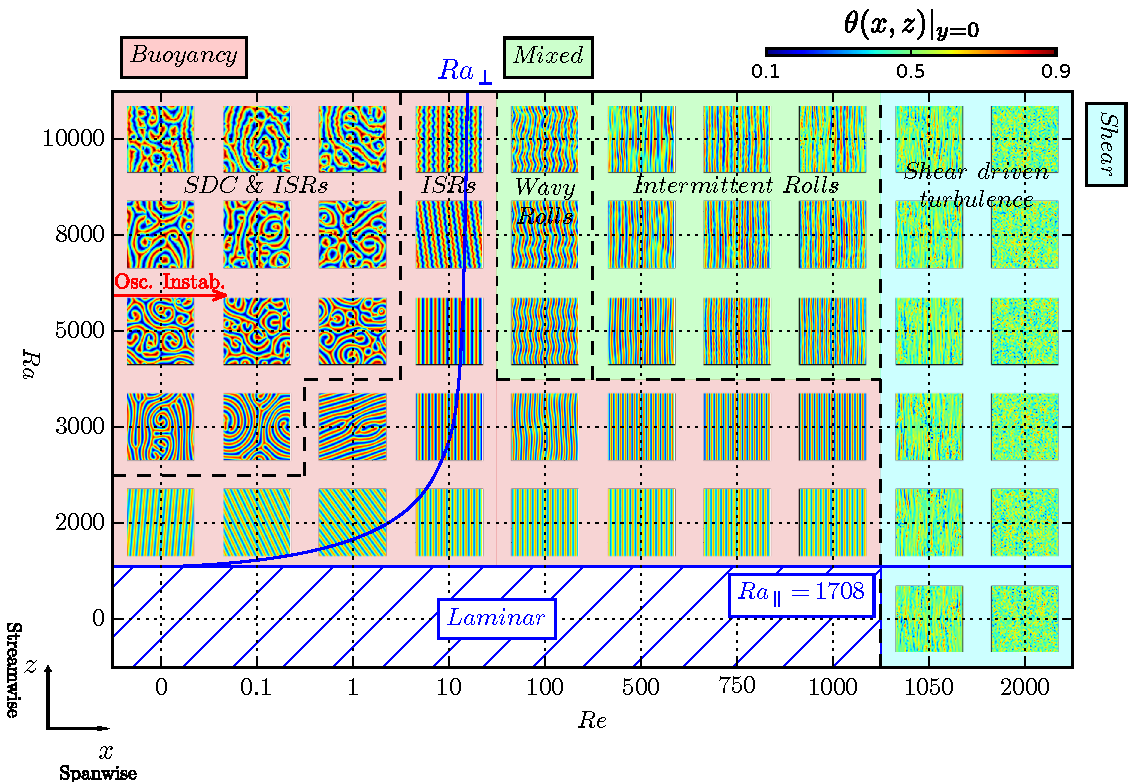
\includegraphics[width=1.3\textwidth, angle=90]{TransitionalRBP/Figures/PhaseSpace/RaRePhaseSpace.pdf}
    \caption{A $Ra-Re$ phase space illustrates the midplane temperature snapshots, $\theta(x,z)|_{y=0}$ for $Re \in [0,2000]$ and $Ra \in [0, 10000]$, $\Gamma = 4\pi$, classified into five distinct regimes: (1) SDC \& ISRs, (2) ISRs, (3) wavy rolls, (4) intermittent rolls and (5) shear-driven turbulence. The blue solid curves refer to primary neutral curves of the longitudinal and transverse rolls $Ra_\parallel, Ra_\perp$. The red arrow indicates the secondary oscillatory instability of ISRs at $Re = 0$, $Ra \sim 6000$ \citep{bodenschatz_recent_2000}. Shades of red, green and blue indicate their dominant mechanism, whether driven by buoyancy or shear (or mixed). For $Re > 0$, the mean flow is along the $z$ direction.}
    \label{fig:rarephase}
\end{figure}

We present the results obtained from the DNS of transitional RBP flows, focusing on the parameter space defined by Rayleigh numbers in the range $Ra \in [0, 10000]$, and Reynolds numbers in the range of $Re \in [0, 2000]$ (see Appendix \ref{app:params} for the full details).

For all numerical simulations, the initial condition consists of a Gaussian white noise with zero mean and unit variance, superimposed onto the laminar base state (i.e. conduction state at $Re = 0$).
The RBP system is then time-integrated untila statistically stationary state is reached, which typically requires a time of $t = O(10)$ to $O(10^2)$.
At the two endpoints of the $Re$-spectrum considered (i.e. $Re = 0, 2000$), SDC and subcritical shear-driven turbulence appear.
Figure \ref{fig:rarephase} shows snapshots of the midplane temperature, $\theta(x,z)|_{y=0}$, of different flow regimes in the $Ra$-$Re$ phase space.
The solid blue curves represent the neutral stability boundaries for the longitudinal and transverse rolls as $Ra_\parallel = 1708$ and $Ra_\perp = f(Re)$, respectively \citep{gage_stability_1968}.
In the absence of shear at $Re=0$, these curves merge into the classical critical RBC instability at $Ra_{c} = 1708$, as ISRs become rotationally invariant about the wall-normal axis.
ISRs may undergo secondary instability for $Ra > Ra_{\parallel}$, and an approximate boundary of this is indicated by a red arrow, roughly indicating the secondary neutral stability boundary, marking the onset of oscillatory instabilities of ISRs within $Ra \gtrsim 5000$ \citep{clever_transition_1974}.
We note that the phase diagram in figure \ref{fig:rarephase} is not-to-scale plotted, serving as a conceptual reference to distinguish between different flow states and their coarse-grained transition boundaries.

In this $Ra$-$Re$ phase space, we categorise the flow behaviour into five distinct regimes: (1) bistability between SDC and ISRs (SDC \& ISRs), (2) ideal straight rolls (ISRs), (3) wavy rolls, (4) intermittent rolls, and (5) shear-driven turbulence.
The categories are defined based on common flow structures (patterns), and/or dynamical characteristics, ranging from equilibrium solutions to intermittent and chaotic dynamics.
Furthermore, we sort out these states based on their first and second-order statistical properties, where they appear independent of $Re$ in the buoyancy-dominated regime (shaded in red), and $Ra$ in the shear-dominated regime (shaded in blue), discussed in detail in  Appendices \ref{app:buoyancy} and \ref{app:shear} respectively.
In the mixed regime shaded in green, both $Ra$ and $Re$ are important.

\begin{figure}[h]
    \centering
    \includegraphics[width=0.8\linewidth]{TransitionalRBP/Figures/PhaseSpace/Ra3kplots.pdf}
    \caption{Midplane temperature snapshots at $Ra = 3000$, (a) $Re = 0.1$, (b) $Re = 1$, (c) $Re = 10$, (d) $Re = 100$, (e) $Re = 1000$, (f) $Re = 2000$.}
    \label{fig:Ra3k}
\end{figure}
Given that the buoyancy-dominated regime is relatively well studied (RBC flow, in particular), we will only provide a brief description of the simulation results in this regime, with further magnified flow fields shown in figure \ref{fig:Ra3k}.
In the buoyancy-dominated regime, the flow structures are predominantly organised with convection rolls, such as SDC, transverse, oblique, longitudinal rolls (and ISRs with no mean flow), or oscillatory rolls.
The bistability between SDC and ISRs (refer to figure \ref{fig:Ra3k}(a)) is preserved for $Ra \geq 3000$ at $Re = 0.1$  and $Re = 1$ for $Ra \geq 5000$ (see also figure \ref{fig:buoyancy_wavy_regime}(a,d,g)). There exists a maximum $Re$, beyond which SDC disappears, we denote this as $Re_s$, and its dependence on $Ra$ is demarcated by the black dashed lines on the left side of figure \ref{fig:rarephase}.
Notably, an oblique roll with a hook-like defect is observed at $Re = 1$, $Ra = 3000$, shown in figure \ref{fig:Ra3k}(b), reminiscent of the multiple non-ISR states in RBC (see references in \S\ref{sec:bkgrd_RBC}).
At $Re = 10$, the SDC disappears and longitudinal rolls with a spanwise wavenumber of $\alpha d = 2.5$ emerge, illustrated in figure \ref{fig:Ra3k}(c), suggesting that the roll wavenumber is within the stability boundaries of the Busse balloon (see also figure 6 in \citet{bodenschatz_recent_2000}).
As $Re$ is increased further to $1000$, the longitudinal rolls emerge as the preferred solution at $Ra = 2000, 3000$.
The non-dimensionalised spanwise wavenumber of the longitudinal rolls observed at $Ra = 3000$ and $Re = 100, 500$ (not shown) and  $Re=1000$, shown in figure \ref{fig:Ra3k}(d-e) respectively, is approximately $\alpha d \approx 3.3$, which lies outside of the stability boundaries of the Busse balloon in RBC (see figure 6 in \citet{bodenschatz_recent_2000}).
This suggests that the stability boundaries of the longitudinal rolls may vary with increasing $Re$.
Interestingly, a stable pinched longitudinal roll pattern emerges at $Re = 100$ $Ra = 3000$, reminiscent of a skew-varicose instability shown in figure \ref{fig:Ra3k}(d).
Unlike the secondary skew-varicose instability observed in RBC (which reduces the wavenumber of an unstable ISR by pinching adjacent rolls together, see figure 7 of \citet{bodenschatz_recent_2000}), a stable pinched tertiary state emerges here.
As $Re$ increases to $2000$, shear-driven turbulence emerges, depicted as a featureless temperature field driven by the underlying turbulent fluctuations in figure \ref{fig:Ra3k}(f).

Figure \ref{fig:buoyancy_wavy_regime} presents a detailed analysis of the coarse-grained transition boundaries between SDC and ISRs in the range $Re \in [1, 10]$, and from ISRs to wavy rolls for $Re \in [10, 100]$ across high Rayleigh numbers considered, $Ra \in [5000, 10000]$.
As $Re$ increases from $1$ to $10$, the SDC regime (see figure \ref{fig:buoyancy_wavy_regime}(a,d,g)) vanishes and longitudinal rolls emerge, as shown in figure \ref{fig:buoyancy_wavy_regime}(b,e,h) for $Ra = 10000, 8000, 5000$, respectively.
These longitudinal rolls may undergo short-wavelength modulations, corresponding to the secondary oscillatory instability of RBC occurring above $Ra \gtrsim 5000$ \citep{clever_transition_1974}.
This results in the development of oscillatory longitudinal rolls described by a relative periodic orbit at $Ra= 8000$, and a chaotic state at $Ra = 10000$, shown in figure \ref{fig:buoyancy_wavy_regime}(e,b) respectively.

The footprint of oscillatory convection rolls is also evident in the SDC regime at $Ra = 10000$, $Re = 1$, shown in figure \ref{fig:buoyancy_wavy_regime}(a).
As $Re$ increases from $10$ to $100$, the longitudinal rolls exhibit longer wavelength modulations, indicative of the wavy instability \citep{clever_instabilities_1991, pabiou_wavy_2005}.
This gives rise to wavy longitudinal rolls, appearing as a travelling wave, quasi-periodic tori, and a chaotic state at $Ra = 5000, 8000, 10000$, shown in figure \ref{fig:buoyancy_wavy_regime}(i,f,c) respectively.
The wavelengths of the streamwise waviness and the spanwise periodic longitudinal roll appear to be approximately $1/3$ of the streamwise length, and $1/12$ of the spanwise length, respectively.
Hence, the ratio between the streamwise waviness wavelength and the spanwise roll is about $4$, consistent with the ratio observed by \citet{clever_instabilities_1991}.


\begin{figure}
    \centering
    \includegraphics[width=1.2\linewidth, angle=90]{TransitionalRBP/Figures/PhaseSpace/BuoyancyRegime-minimal.pdf}
    \caption{The space-time plots of midplane temperature field, temperature snapshot and phase space trajectories of the Nusselt number against wall shear rate at  (a,b,c) $Ra = 10000$ for $Re = 1, 10, 100$; (d,e,f) $Ra = 8000$ for $Re = 1,10,100$; and (g,h,i) $Ra = 5000$ for $Re = 1, 10, 100$. The flow patterns are primarily organised into spiral defect chaos, longitudinal rolls, and wavy rolls occurring at $Re = 1, 10, 100$, respectively.}
    \label{fig:buoyancy_wavy_regime}
\end{figure}

\subsection{Spatiotemporal intermittent rolls}\label{sec:intermittentrolls}
\begin{figure}
    \centering
    \includegraphics[width=\linewidth]{TransitionalRBP/Figures/PhaseSpace/Ra8000-Re500-BotSpaceTime-TimeHist.pdf}
    \caption{The intermittent rolls regime at $Ra = 8000, Re = 500$, $t \in [0, 10000]$. (a) The time history of shear on the lower wall and the Nusselt number. Space-time ($x$-$t$) plots of (b) near-wall wall-normal and spanwise perturbation kinetic energy and (c) midplane temperature space-time plot, with the corresponding near-wall and midplane temporal planar snapshots at (d,e) $t = 3736$, (f,g) $t = 6189$, and (h,i) $t = 8680$.}
    \label{fig:Ra8k-Re500-IntRolls}
\end{figure}

As $Re$ approaches $Re = 500$, the wavy rolls disappear.
Instead, a new regime, referred to as intermittent rolls, is observed.
In this regime, the longitudinal rolls remain as the dominant convection structure, interspersed with a spatio-temporal intermittent breakdown towards the laminar state.
This behaviour is illustrated for $(Ra, Re) = (8000,500$) in figure \ref{fig:Ra8k-Re500-IntRolls}(a) using the temporal oscillations of the plane-averaged shear rate on the lower wall, $\langle \tau_w \rangle_{x,z}$, and the Nusselt number, $Nu$. 
We note that $\tau_w = 2$ and $Nu = 1$ for the laminar solution.

The spatio-temporal intermittent breakdown of the longitudinal rolls towards the laminar state is observed in figure \ref{fig:Ra8k-Re500-IntRolls}(b), where the bright and dark regions in the space-time plot of near-wall spanwise and wall-normal perturbation kinetic energy ($\mathcal{E}_{u'+v'} = 1/2(u'^2+ v'^2)$) at $(y^+,z)=(15,8\pi)$, highlight the co-existence of longitudinal rolls and spatially localised laminar states; here, $\mathbf{u}' = \mathbf{u} - W_{lam}(y)$ and $y^+ \equiv (y+1)/Re_\tau$ with $Re_\tau \equiv u_\tau h/\nu$, where $u_\tau$ is the friction velocity.
A similar observation is made with the space-time plot of midplane temperature, $\theta|_{(y,z)=(0,8\pi)}$, in figure \ref{fig:Ra8k-Re500-IntRolls}(c), where the elongated red/blue contours correspond to up-/down-welling regions of longitudinal rolls, and the green regions indicate spatially-localised laminar states.
The two near-wall transport properties, the wall shear rate and the Nusselt number, exhibit strong correlations.
For example, at $t = 3736$, both peaks reveal a spatially coherent longitudinal roll structure in figure \ref{fig:Ra8k-Re500-IntRolls}(d,e). There are also dips observed at $t = 6189$ and $t=8680$, indicative of the spatially local breakdown towards the laminar state, as shown in figures \ref{fig:Ra8k-Re500-IntRolls}(f,g) and \ref{fig:Ra8k-Re500-IntRolls}(h,i), respectively.
In summary, the longitudinal rolls enhance heat and momentum transfer towards the walls, but they appear to be intermittently disrupted by the breakdown towards the laminar state.
To better understand this behaviour, we later consider the temporal dynamics in a confined domain, $\Gamma = \pi / 2$, where the spatial intermittency is artificially suppressed (see \S \ref{sec:TASP}).

\subsection{Co-existence of convection rolls with turbulent bands}\label{sec:rbp_3.3}
\begin{figure}
\centering
\includegraphics[width=\linewidth]{TransitionalRBP/Figures/RaEffectOnTurbulence/Ra0-Re1050-3-BotSpaceTime-Lows.pdf}
\caption{Shear-driven turbulence regime at $Ra = 0, Re = 1050$, $t \in [0, 8000]$. Space-time plots of (a) near-wall wall-normal and spanwise perturbation kinetic energy, (b) midplane temperature space-time plot, and near-wall and midplane temporal planar snapshots at (c,d) $t = 1100$, (e,f) $t = 4491$, and (g,h) $t = 6171$, highlighting a prolonged laminar patch.}
\label{fig:spacetime-Ra0k-Re1.05k}
\end{figure}

As $Re$ approaches $Re = 1050$, shear-driven turbulence emerges as spatio-temporal intermittent turbulent-laminar bands, where turbulent and laminar regions can co-exist \citep{tuckerman_patterns_2020}.
In the absence of buoyancy (i.e. $Ra = 0$), these bands emerge clearly shown in figure \ref{fig:spacetime-Ra0k-Re1.05k}.
The space-time plot of the near-wall wall-normal and spanwise perturbation kinetic energy, $\mathcal{E}_{u'+v'}$ (here we use wall units to illustrate the near-wall turbulent streaks), at $y^+ = 15$ in figure \ref{fig:spacetime-Ra0k-Re1.05k}(a) highlights this co-existence, where the turbulent and laminar regions are indicated by dark and bright areas, respectively.
In particular, a period of prolonged laminar state is observed at $t = 1100, 4491, 6171$, represented by localised green regions in the space-time plot of midplane temperature, $\theta|_{(y,z)=(0,8\pi)}$, in figure \ref{fig:spacetime-Ra0k-Re1.05k}(b).
The prolonged laminar states are also evident in the near-wall and midplane temporal snapshots of figures \ref{fig:spacetime-Ra0k-Re1.05k}(c-h), shown as large pockets of dark and green regions that fill approximately half of the spatial domain.

\begin{figure}
\centering
\includegraphics[width=\linewidth]{TransitionalRBP/Figures/RaEffectOnTurbulence/Ra10000-Re1050-BotSpaceTime-Highs.pdf}
\caption{Shear-driven turbulence regime at $Ra = 10000, Re = 1050$, $t \in [0, 8000]$. Space-time plots of (a) near-wall wall-normal and spanwise perturbation kinetic energy, (b) midplane temperature spacetime plot, and their corresponding near-wall and midplane temporal $x-z$ planar snapshots at (c,d) $t = 1282$, (e,f) $t = 5077$, and (g,h) $t = 6358$, highlighting the coexistence of longitudinal rolls and turbulent bands.}
\label{fig:spacetime-Ra10k-Re1.05k}
\end{figure}

Next, we consider the influence of buoyancy on the turbulent-laminar bands and compare two distinctly different cases of buoyancy using $Ra = 0$ and $Ra = 10000$ at $Re = 1050$.
In the latter case, the typical features of the turbulent-laminar bands depicted as alternate dark and bright bands are also seen in the space-time plot of near-wall wall-normal and spanwise perturbation kinetic energy, $\mathcal{E}_{u'+v'}$, in figure \ref{fig:spacetime-Ra10k-Re1.05k}(a).
However, some important differences emerge compared to the former case (in $Ra = 0$).
In particular, the midplane temperature snapshots, $\theta|_{(y,z)=(0,8\pi)}$, at $t = 1282, 5077, 6358$ in figures \ref{fig:spacetime-Ra10k-Re1.05k}(d,f,h) reveal some localised regions of streamwise-aligned red and blue contour stripes, likely indicating the presence of longitudinal rolls.
These longitudinal roll regions are typically located next to neighbouring turbulent (bright) regions in the near-wall perturbation kinetic energy snapshots in figures \ref{fig:spacetime-Ra10k-Re1.05k}(c,e,g), suggesting that longitudinal rolls co-exist with turbulent patches at $Ra = 10000$.
However, we caution that although they are relatively weak, similar red and blue contour stripes are also observed at $Ra = 0$, where longitudinal rolls are not expected, as shown in figure \ref{fig:spacetime-Ra0k-Re1.05k}(f). In this case, these weak elongated red and blue contour stripes are likely to be from the near-wall streaks.

Nonetheless, turbulence occurs more spatially intermittently at $Ra = 0$, containing prolonged pockets of laminar regions, while turbulent regions at $Ra = 10000$ appear more visibly consistently (compare figures \ref{fig:spacetime-Ra0k-Re1.05k}a with \ref{fig:spacetime-Ra10k-Re1.05k}a).
In other words, the presence of longitudinal rolls may promote turbulence locally, and we will investigate this issue further in \S \ref{sec:rbp_4}.

\section{The role of longitudinal rolls}\label{sec:rbp_4}
\subsection{The thermally-assisted sustaining process (TASP) in a confined domain}\label{sec:TASP}
\begin{figure}
    \centering
    \includegraphics[width=\linewidth]{TransitionalRBP/Figures/RaEffectOnTurbulence/Ra10000-Re1050-MidBotTimeHist-4x4.png}
    \caption{Intermittent dynamics in a confined domain at $Ra = 10000$, $Re = 1050$, $t\in[0,3000]$, $\Gamma = \pi/2$. The time history of the (a) Nusselt number and shear. Temporal snapshots of volumetric temperature, planar near-wall streamwise and spanwise perturbations at (b) $t = 1291.5$, (c) $t = 1480.5$, (d) $t = 1564.5$, (e) $t = 1711.5$. Longitudinal rolls and transient turbulence are observed at (b,d) and (c,e), respectively.}
    \label{fig:Ra10k-Re1050-small}
\end{figure}

Given the complexities in the spatio-temporal dynamics observed in \S\ref{sec:rbp_3},
we consider simulations confined to a domain defined by $\Gamma = \pi/2$, where longitudinal rolls and localised turbulence could be viewed as spatially isolated.
We start from a numerical simulation at $Ra = 10000$ and $Re=1050$ in $\Gamma = \pi/2$, integrated in time for $t \in [0, 3000]$. 
The initial condition has been sampled from a statistically stationary turbulent field at $Re = 2000$ for $Ra=10000$, and the $Re$ is then slowly lowered to $Re = 1050$.
The time history for $t \in [0, 3000]$ of the two near-wall transport properties, the Nusselt number and the shear rate on the lower wall, is presented in figure \ref{fig:Ra10k-Re1050-small}, together with snapshots of the temperature, $\theta(\mathbf{x})$, and the near-wall streamwise and spanwise perturbation velocities, $w'|_{y^+= 15}, v'|_{y^+=15}$ at selected times.
In this confined domain, the dynamics of the system exhibit temporal intermittency, where the solution trajectory appears to wander between longitudinal rolls and highly disorganised chaotic flow fields, characterised by low- and high-near-wall transport properties, respectively.

Starting from a longitudinal roll state of spanwise wavenumber of $\alpha d = 4$ at $t = 1291.5$ in figure \ref{fig:Ra10k-Re1050-small}(b), the solution erupts into a highly disorganised turbulent state at $t = 1480.5$, marked by a disordered temperature field in figure \ref{fig:Ra10k-Re1050-small}(c).
During this breakdown, the near-wall snapshots of streamwise perturbation velocity, $w'|_{y^+ = 15}$, and wall-normal perturbation velocity, $v'|_{y^+ = 15}$, illustrated in the bottom panels of figures \ref{fig:Ra10k-Re1050-small}(c), reveal three pairs of high- and low-speed streaks, each with an average spanwise wavelength of $\Lambda_x^+ \approx 339/3 = 113$ (where $\Lambda_x^+ = u_\tau \Lambda_x / \nu$ is the non-dimensionalised wavelength by wall units), close to the mean streak spacing ($\Lambda^+_x \sim 100$) commonly reported in shear flow turbulence \citep{kline_structure_1967, kim_turbulence_1987, hamilton_regeneration_1995}.
These streaks appear to be meandering, negatively correlated with wall-normal perturbation velocities, reminiscent of a streak breakdown process \citep{hamilton_regeneration_1995}, or a bursting event \citep{kim_production_1971}, where high (low)-speed streaks are brought close to (away from) the wall, enhancing near-wall transport quantities.
The enhancement is reflected in large increments in the Nusselt number and wall shear rate of roughly $40\%$ at $t = 1480.5$ in figure \ref{fig:Ra10k-Re1050-small}(a).
Subsequently, the solution trajectory returns to a longitudinal roll state at $t=1564.5$, before erupting into turbulence at $t = 1711.5$ (see figures \ref{fig:Ra10k-Re1050-small}(d,e) respectively).
This suggests that the turbulence has a finite lifetime, occurring transiently before decaying towards the laminar state at $Re = 1050$ \citep{hof_finite_2006, schneider_turbulence_2007}, which is linearly unstable, leading to the onset of longitudinal rolls where transient turbulence could be re-excited again.

\begin{figure}
    \centering
    \includegraphics[width=\linewidth]{TransitionalRBP/Figures/RaEffectOnTurbulence/Ra0-Re1050-MidBotTimeHist.png}
    \caption{Relaminarisation in a confined domain at $Ra = 0$, $Re = 1050$, $t\in[0,3000]$, $\Gamma = \pi/2$. The time history of the (a) Nusselt number and shear. Temporal snapshots of volumetric temperature at (b) $t = 31.5$, (c) $t = 63$, (d) $t = 157.5$, (e) $t = 672$.}
    \label{fig:Ra0k-Re1050-small}
\end{figure}

To test this hypothesis, we consider a numerical simulation at $Ra = 0$, $Re = 1050$, in $\Gamma = \pi / 2$, where longitudinal rolls cannot appear.
The initial condition is taken from a stationary turbulent solution at a higher $Re$ of $Re = 2000$, which is then slowly lowered to $Re = 1050$, and then integrated in time for $t \in [0, 700]$.
The time history of the Nusselt number, $Nu$, and the wall shear rate, $\langle \tau_w \rangle_{x,z}$, is reported in figure \ref{fig:Ra0k-Re1050-small}, with the temperature snapshots, $\theta(\mathbf{x})$, at selected time units. 
An initial turbulent flow field decays towards the laminar solution in $t \in [0, 700]$.
Comparing the results between $Ra = 0$ and $Ra = 10000$, we propose that the longitudinal rolls at $Ra= 10000$ could mediate a transition mechanism between unstable laminar state and transient turbulence, so that the entire nontrivial flow dynamics could be sustained indefinitely.

\begin{figure}
    \centering
    \includegraphics[width=\linewidth]{TransitionalRBP/Figures/RaEffectOnTurbulence/T1620-MidBotTimeHist-Quenched-Annotated.pdf}
    \caption{$Ra$-quenching experiments for $Ra = 8000, 5000, 3000, 2000$, at $Re = 1050$, $\Gamma = \pi/2$, $t \in [850.5, 5000]$. The time history of (a) shear and (b) volumetric temperature snapshots of the flow condition at $t = 850.5$. Volumetric temperature snapshots for $Ra = 8000$ at (c,d) $t = 1312.5, 1743$, and $Ra = 5000$ at (e,f) $t = 1312.5, 3570$, revealing a longitudinal roll and a turbulent state, respectively. Stable longitudinal rolls emerge for $Ra = 3000$ at (g,h) $t = 1312.5, 4200$, and $Ra = 2000$ at (j,k) $t = 1312.5, 4200$.}
    \label{fig:RaQuench}
\end{figure}

Next, we investigate the impact of longitudinal rolls on this proposed mechanism at different $Ra$.
We save the flow for $Ra=10000$ and $Re=1050$ at $t=850.5$ (just before the onset of longitudinal rolls, see figure \ref{fig:Ra10k-Re1050-small}), and use the flow as an initial condition to perform four numerical simulations by lowering $Ra$ instantly to $Ra=8000,5000,3000,2000$, respectively, and we then time-integrated further to $t \in [850.5, 5000]$.
The time history of the wall shear rate, $\langle \tau_w\rangle_{x,z}$, and the temperature snapshots, $\theta(\mathbf{x})$, of these experiments of $Ra$-quenching are presented in figure \ref{fig:RaQuench}.
The time history of shear is visibly intermittent for $Ra = 8000, 5000$, depicted as the orange and green trajectories in figure \ref{fig:RaQuench}(a), similar to $Ra = 10000$.
At $Ra= 8000, 5000$, the longitudinal rolls emerge approximately at $t = 1312.5$ (see figures \ref{fig:RaQuench}(c,e)), before erupting into turbulence at $t = 1743$ and $t = 3570$ in figures \ref{fig:RaQuench}(d,f), respectively.
This is then accompanied by a large spike in the wall shear rate before dipping briefly, shown as the orange and green trajectories of figure \ref{fig:RaQuench}(a).
As $Ra$ is lowered further to $Ra = 3000, 2000$, the transients begin to decay into a longitudinal state from $t = 850.5$ to $t = 1312.5$, which remains stable until $t = 4200$ illustrated by figure \ref{fig:RaQuench}(h,j), accompanied by the red and purple asymptotic trajectories in figure \ref{fig:RaQuench}(a). 
This suggests that the longitudinal rolls are likely to be linearly unstable for $Ra = 8000, 5000$, leading to turbulence, while remaining stable for $Ra = 3000,2000$.
In particular, the longitudinal roll state at $Ra = 5000$ remained saturated for a longer period $t \in [1500, 3400]$ (green curve in figure \ref{fig:RaQuench}(a)), indicating that the growth rate of the linear instability is smaller than for $Ra =  8000$.
We note that the longitudinal rolls in figure \ref{fig:RaQuench} have a spanwise wavenumber of $\alpha d=4$, which corresponds to the wavenumber of the dominant primary instability (see Appendix \ref{app:long-pri}), indicating that it is the most preferred wavenumber within the confined domain.

\begin{figure}
    \centering
    \includegraphics[width=\linewidth]{TransitionalRBP/Figures/RaEffectOnTurbulence/ev-compiled.pdf}
    \caption{The growth rates of infinitesimal perturbations linearised about longitudinal rolls, $\mathbf{q}_{LR}$, of spanwise wavenumber of $\alpha d = 4$, against (a) streamwise wavenumber $\beta d$, and (b) $Ra$ for $\beta d =2$. The hatches in (a) refer to wavenumbers smaller than those admissible in $\Gamma = \pi/2$. The dash-dotted line in (b) is a standard quadratic regression yielding $Ra_{s}\approx 4720$.}
    \label{fig:SecStabLongRolls}
\end{figure}

To understand the stability characteristics of the longitudinal rolls, we perform a linear stability analysis about the longitudinal roll state ($\alpha d= 4$), at $Ra = 10000, 8000, 5000, 3000, 2000$.
The details of linear stability analysis are described in \S\ref{sec:linearstab}, where $\lambda$ and $\mathbf{\breve{q}}(x,y)e^{i\beta z}$ refer to the eigenvalue and eigenmode.
The longitudinal roll (base) states, $\mathbf{q}_{LR}$, are obtained by time integrating an initial condition consisting of the laminar (conduction) state, superimposed by the primary eigenmode, $\alpha d = 4$, at $Ra = 10000, 8000, 5000, 3000, 2000$, in a two-dimensional $x-y$ plane, suppressing any three-dimensional perturbations numerically.
The growth rates as a function of discrete streamwise wavenumbers, $2 \leq \beta d \leq 5$, are presented in figure \ref{fig:SecStabLongRolls}.
We note that the admissible streamwise wavenumbers within $\Gamma = \pi/2$ are $\beta d = m$, where $m$ is a positive even integer, $m = 2, 4, ..$, and $\beta d = 3, 5$ are included for completeness.
The longitudinal rolls are linearly unstable for $Ra \geq 5000$, while they remain stable for $Ra \leq 3000$, which confirms our hypothesis earlier. 
In particular, the growth rates between $Ra = 5000$ and $Ra = 10000$ differ by an order of magnitude, which could explain the prolonged period of saturation in the green curve of figure \ref{fig:RaQuench}(a).
The dominant secondary instability of longitudinal rolls in $\Gamma = \pi / 2 $ has a streamwise wavenumber of $\beta d = 2$.
Using a standard quadratic regression, the critical Rayleigh number for disturbances with $\beta d = 2$ is approximately $Ra_{s} \approx 4720$, presented in figure \ref{fig:SecStabLongRolls}(b).

\begin{figure}
    \centering
    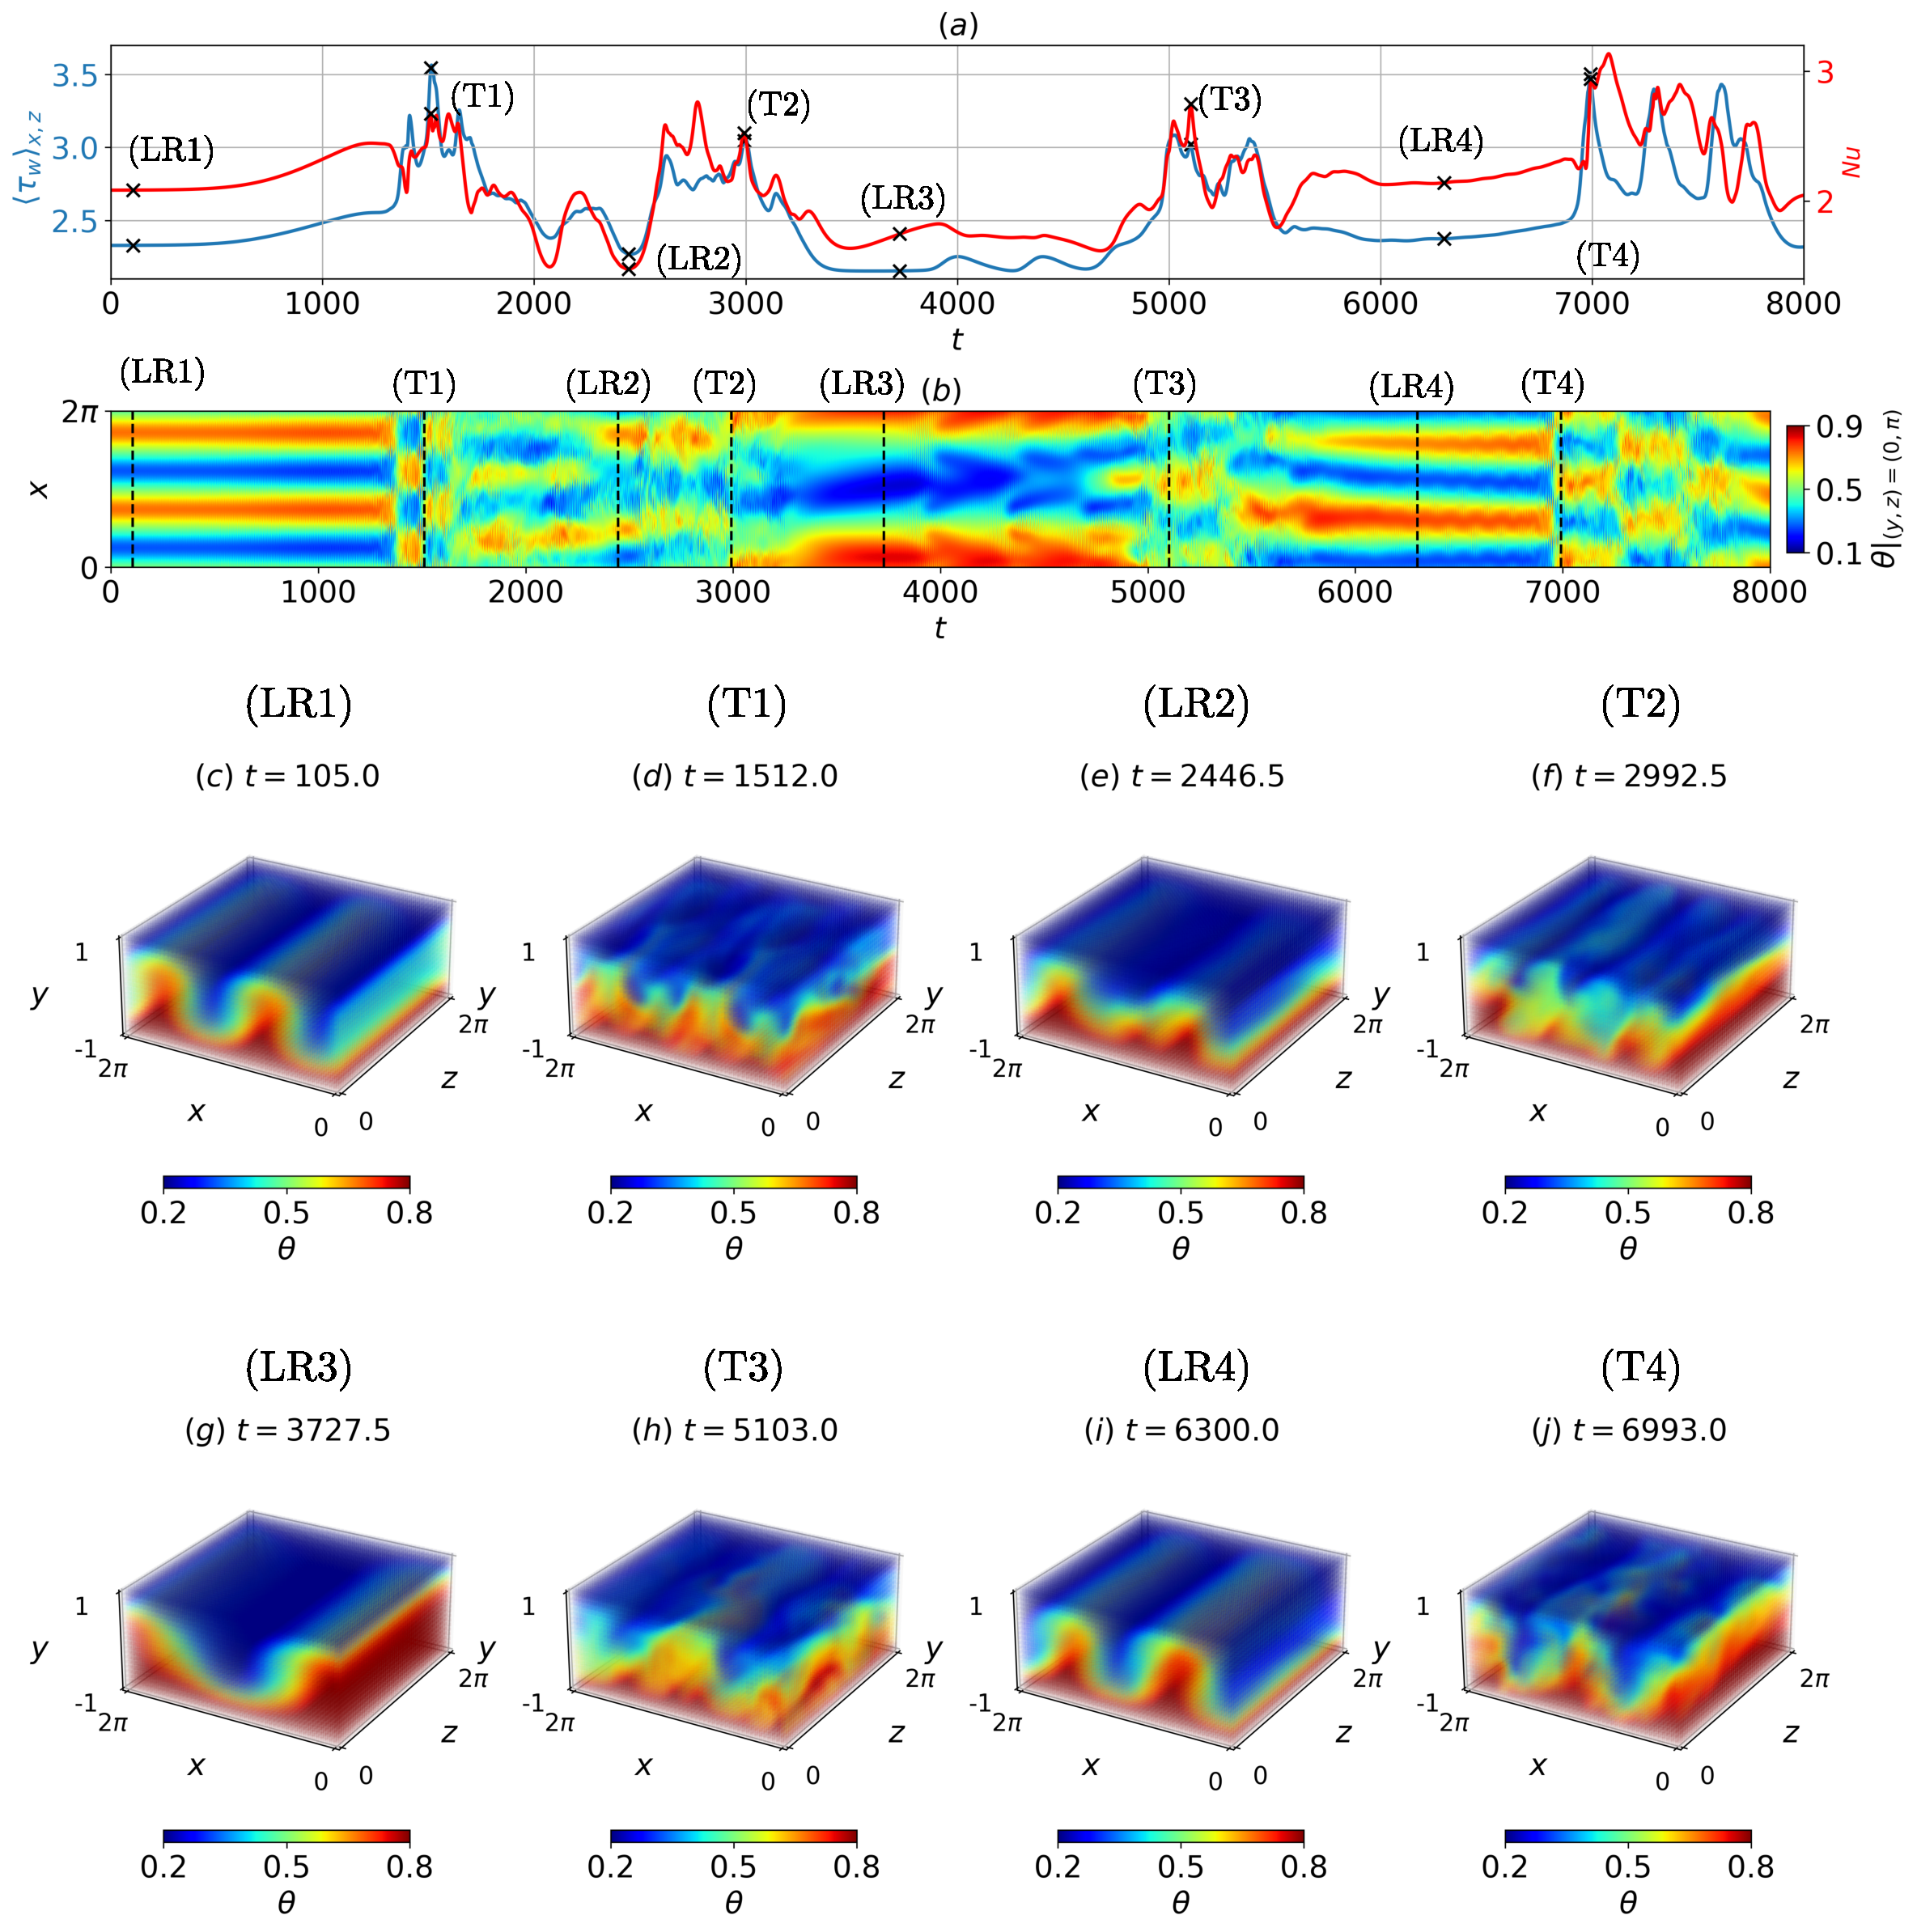
\includegraphics[width=\linewidth]{TransitionalRBP/Figures/RaEffectOnTurbulence/Ra5000-Re1050-MidBotTimeHist-PEig-minimal-labelled.pdf}
    \caption{Time integration along the dominant unstable eigenmode, $\beta d =2$, of the longitudinal rolls at $Ra = 5000, Re = 1050, \Gamma = \pi/2$ for $t\in[0,8000]$. Time history of the (a) Nusselt number and wall shear rate, and (b) midplane temperature space-time plot. This system oscillates between the longitudinal rolls ($LR1-4$) and turbulence ($T1-4$) over four intervals. Snapshots of temperature at (c) $t = 105$, (d) $t = 1512$, (e) $t = 2446.5$, (f) $t = 2992.5$, (g) $t = 3727.5$, (h) $t = 5103$, (i) $t = 6300$, (j) $t = 6993$.}
    \label{fig:intermittent-dynamics}
\end{figure}

Following this, we examine the dominant unstable eigenmode ($\beta d = 2$) of the longitudinal rolls ($\alpha d = 4$) at $Ra=5000$, by considering an initial condition
\begin{equation}\label{eq:SecInstab}
\mathbf{q}_0(\mathbf{x},t=0) = \mathbf{q}_{LR}(x,y) + (\mathbf{\breve{q}}(x,y)e^{i\beta z}+c.c).
\end{equation}
Here, $\breve{\mathbf{q}} e^{i\beta z}$ is an eigenmode for the streamwise wavenumber $\beta$, and its amplitude was scaled such that its total energy is
\begin{equation}\label{eq:totalenergy}
\delta \equiv \frac{1}{{V}} \int_\Omega (\mathbf{\hat{u}}(\mathbf{x})^T\mathbf{\hat{u}}(\mathbf{x}) + \frac{Ra}{8Re^2Pr}\hat{\theta}(\mathbf{x})^2 )\; \mathrm{d}\Omega = 10^{-3}.
\end{equation}
We have also considered $\delta = 10^{-2}, 10^{-4}$, but $\delta = 10^{-3}$  was found to be small enough to ensure linear growth while large enough without requiring a large number of time steps.

The initial condition is time-integrated for $t \in [0, 8000]$, and the time history of the near-wall transport properties, the space-time plot of the mid-plane temperature, $\theta|_{(y,z)=(0,\pi)}$, are presented in figure \ref{fig:intermittent-dynamics}, with snapshots of temperature, $\theta(\mathbf{x})$, and near-wall streamwise and spanwise perturbation velocities, $w'|_{y^+= 15}, v'|_{y^+=15}$ at some selected times. 
The intermittent trajectory is visually apparent, oscillating between longitudinal rolls and transient turbulence over four cycles for $t \in [0, 8000]$: for example, the regions of low and high near-wall transport quantities in figure \ref{fig:intermittent-dynamics}(a) correspond well to the organised and disorganised longitudinal rolls in figure \ref{fig:intermittent-dynamics}(b), respectively.
As the solution emerges from the unstable eigenmode of the longitudinal roll state, $(LR1)$ in figure \ref{fig:intermittent-dynamics}(c), the trajectory erupts into turbulence at $t = 1512$, marked by a disordered volumetric temperature field in snapshot $(T1)$ in figure \ref{fig:intermittent-dynamics}{\color{blue}(d)}.
Turbulence occurs transiently, and the solution decays towards a longitudinal roll-like state at $t = 2446.5$, shown by snapshot $(LR2)$ in figure \ref{fig:intermittent-dynamics}(e), forming a single cycle.
The intermittent cycle repeats over three subsequent intervals, where the transient turbulent state and longitudinal rolls emerge at $t = 2992.5, 5103, 6993$, and $t = 3727.5, 6300$, as shown in the snapshots $(T2,3,4)$ and $(LR3,4)$ in figures \ref{fig:intermittent-dynamics}(f,h,j) and \ref{fig:intermittent-dynamics}(g,i), respectively.
Lastly, we show that the dominant unstable eigenmode of the longitudinal rolls is connected to a transient turbulent state.
Interestingly, a longitudinal roll with $\alpha d = 2$ sometimes emerges after turbulence decays, shown as the snapshot $(LR3)$.
This suggests that other unstable eigenmodes may well be linked to the transition to transient turbulence.

\begin{figure}
    \centering
    \includegraphics[width=\linewidth]{TransitionalRBP/Figures/RaEffectOnTurbulence/Ra5000-Re1050-StateSpace-dudy.png}
    \caption{State space projection based on the planar averaged centerline velocity and shear, coloured by the volume normalised perturbation kinetic energy at $Ra = 5000$, $Re = 1050$, $\Gamma = \pi/2$, (a) $t \in[0,800]$, (b) $t \in [0, 68750]$.  The open black circles represent the unstable equilibria of longitudinal rolls and the laminar state. Note that the black-crosses, labelled by (T1-4) and (LR1-4), refer to temporal snapshots in figure \ref{fig:intermittent-dynamics}, not equilibria solutions.}
    \label{fig:intermittent-state-space}
\end{figure}

To better visualise the temporal dynamics in figure \ref{fig:intermittent-dynamics}, we project the solution trajectory onto the space composed of two state observables: planar averaged centerline velocity, $\langle w|_{y=0} \rangle _{x,z}$, the wall shear rate, $\langle \tau_w\rangle_{x,z}$ coloured by the volume-averaged perturbation kinetic energy, $1/(2V)||\mathbf{u}'||^2$, in figure \ref{fig:intermittent-state-space}, where $\|\mathbf{u}'\|^2=\int_\Omega \mathbf{u}'^H\mathbf{u}' dV$ with $\Omega$ being the flow domain.
These observables are chosen because they are found to distinguish well the regions of turbulent states, longitudinal roll states, and the laminar state that reside around $(0.82, 3.2)$, $(0.90, 2.32)$, and at $(1, 2)$, respectively. Indeed, the temporal snapshots of $(T1-4)$ appear around the representative location of turbulent states, $(0.82, 3.2)$, and the snapshots of $(LR1-4)$ and an equilibrium related to the longitudinal roll state with the spanwise wavenumber $\alpha d=4$ (denoted by $\mathbf{q}_{LR, \alpha d = 4}$) are seen around $(0.90, 2.32)$.

The solution trajectory emerges from the unstable manifold of the longitudinal roll state, $\mathbf{q}_{LR_{\alpha d = 4}}$, evolving towards turbulent states around $(0.85,3.2)$, characterised by a high wall shear rate.
At this $Re$, the turbulence is transient in the confined domain, occurring with a finite lifetime, eventually decaying towards the laminar state \citep{zammert_streamwise_2014, tuckerman_patterns_2020, paranjape_direct_2023}.
As the solution trajectory approaches the laminar solution at $(1,2)$, it abruptly reverses towards the longitudinal roll state near $(0.95, 2.15)$, $(LR3)$ due to the buoyancy-driven linear instability of the laminar base state in the RBP flow. 
Subsequently, the solution trajectory again departs along an unstable eigenmode of the longitudinal rolls, forming a cyclic process.

To see if this cycle could be sustained indefinitely, we consider a longer time horizon, $t \in [0, 68750]$, illustrated in figure \ref{fig:intermittent-state-space}(b).
The solution trajectory wanders between the `cloud' of transient turbulence at the top left corner (in red), and longitudinal roll and laminar states (in blue) in the bottom right, forming a cycle between the unstable longitudinal rolls, transient turbulence, and the unstable laminar base state.
This cycle is likely established above a critical $Ra$ as the longitudinal rolls become linearly unstable (i.e. $Ra \gtrsim Ra_{s} \approx 4720$, see figure \ref{fig:SecStabLongRolls}(b)), and the instability of the longitudinal rolls provides an intermediate pathway towards transient turbulence, which could be regenerated again - a self-sustaining dynamical process.
We refer to this process as the \emph{thermally-assisted sustaining process (TASP)}, inspired by the self-sustaining process (SSP) from turbulent shear flows (see \S \ref{subsec:SSP}).
A schematic of the \textit{TASP} is illustrated in figure \ref{fig:tasp}.

\begin{figure}
    \centering
    \includegraphics[width=0.7\linewidth]{TransitionalRBP/Figures/RaEffectOnTurbulence/TASP-graphics.pdf}
    \caption{The thermally-assisted sustaining process (TASP).}
    \label{fig:tasp}
\end{figure}

\subsection{Variation of $Ra$ and $Re$ on the thermally-assisted sustaining process in $\Gamma = \pi/ 2$}\label{sec:IntConfined}

\begin{figure}
\centering
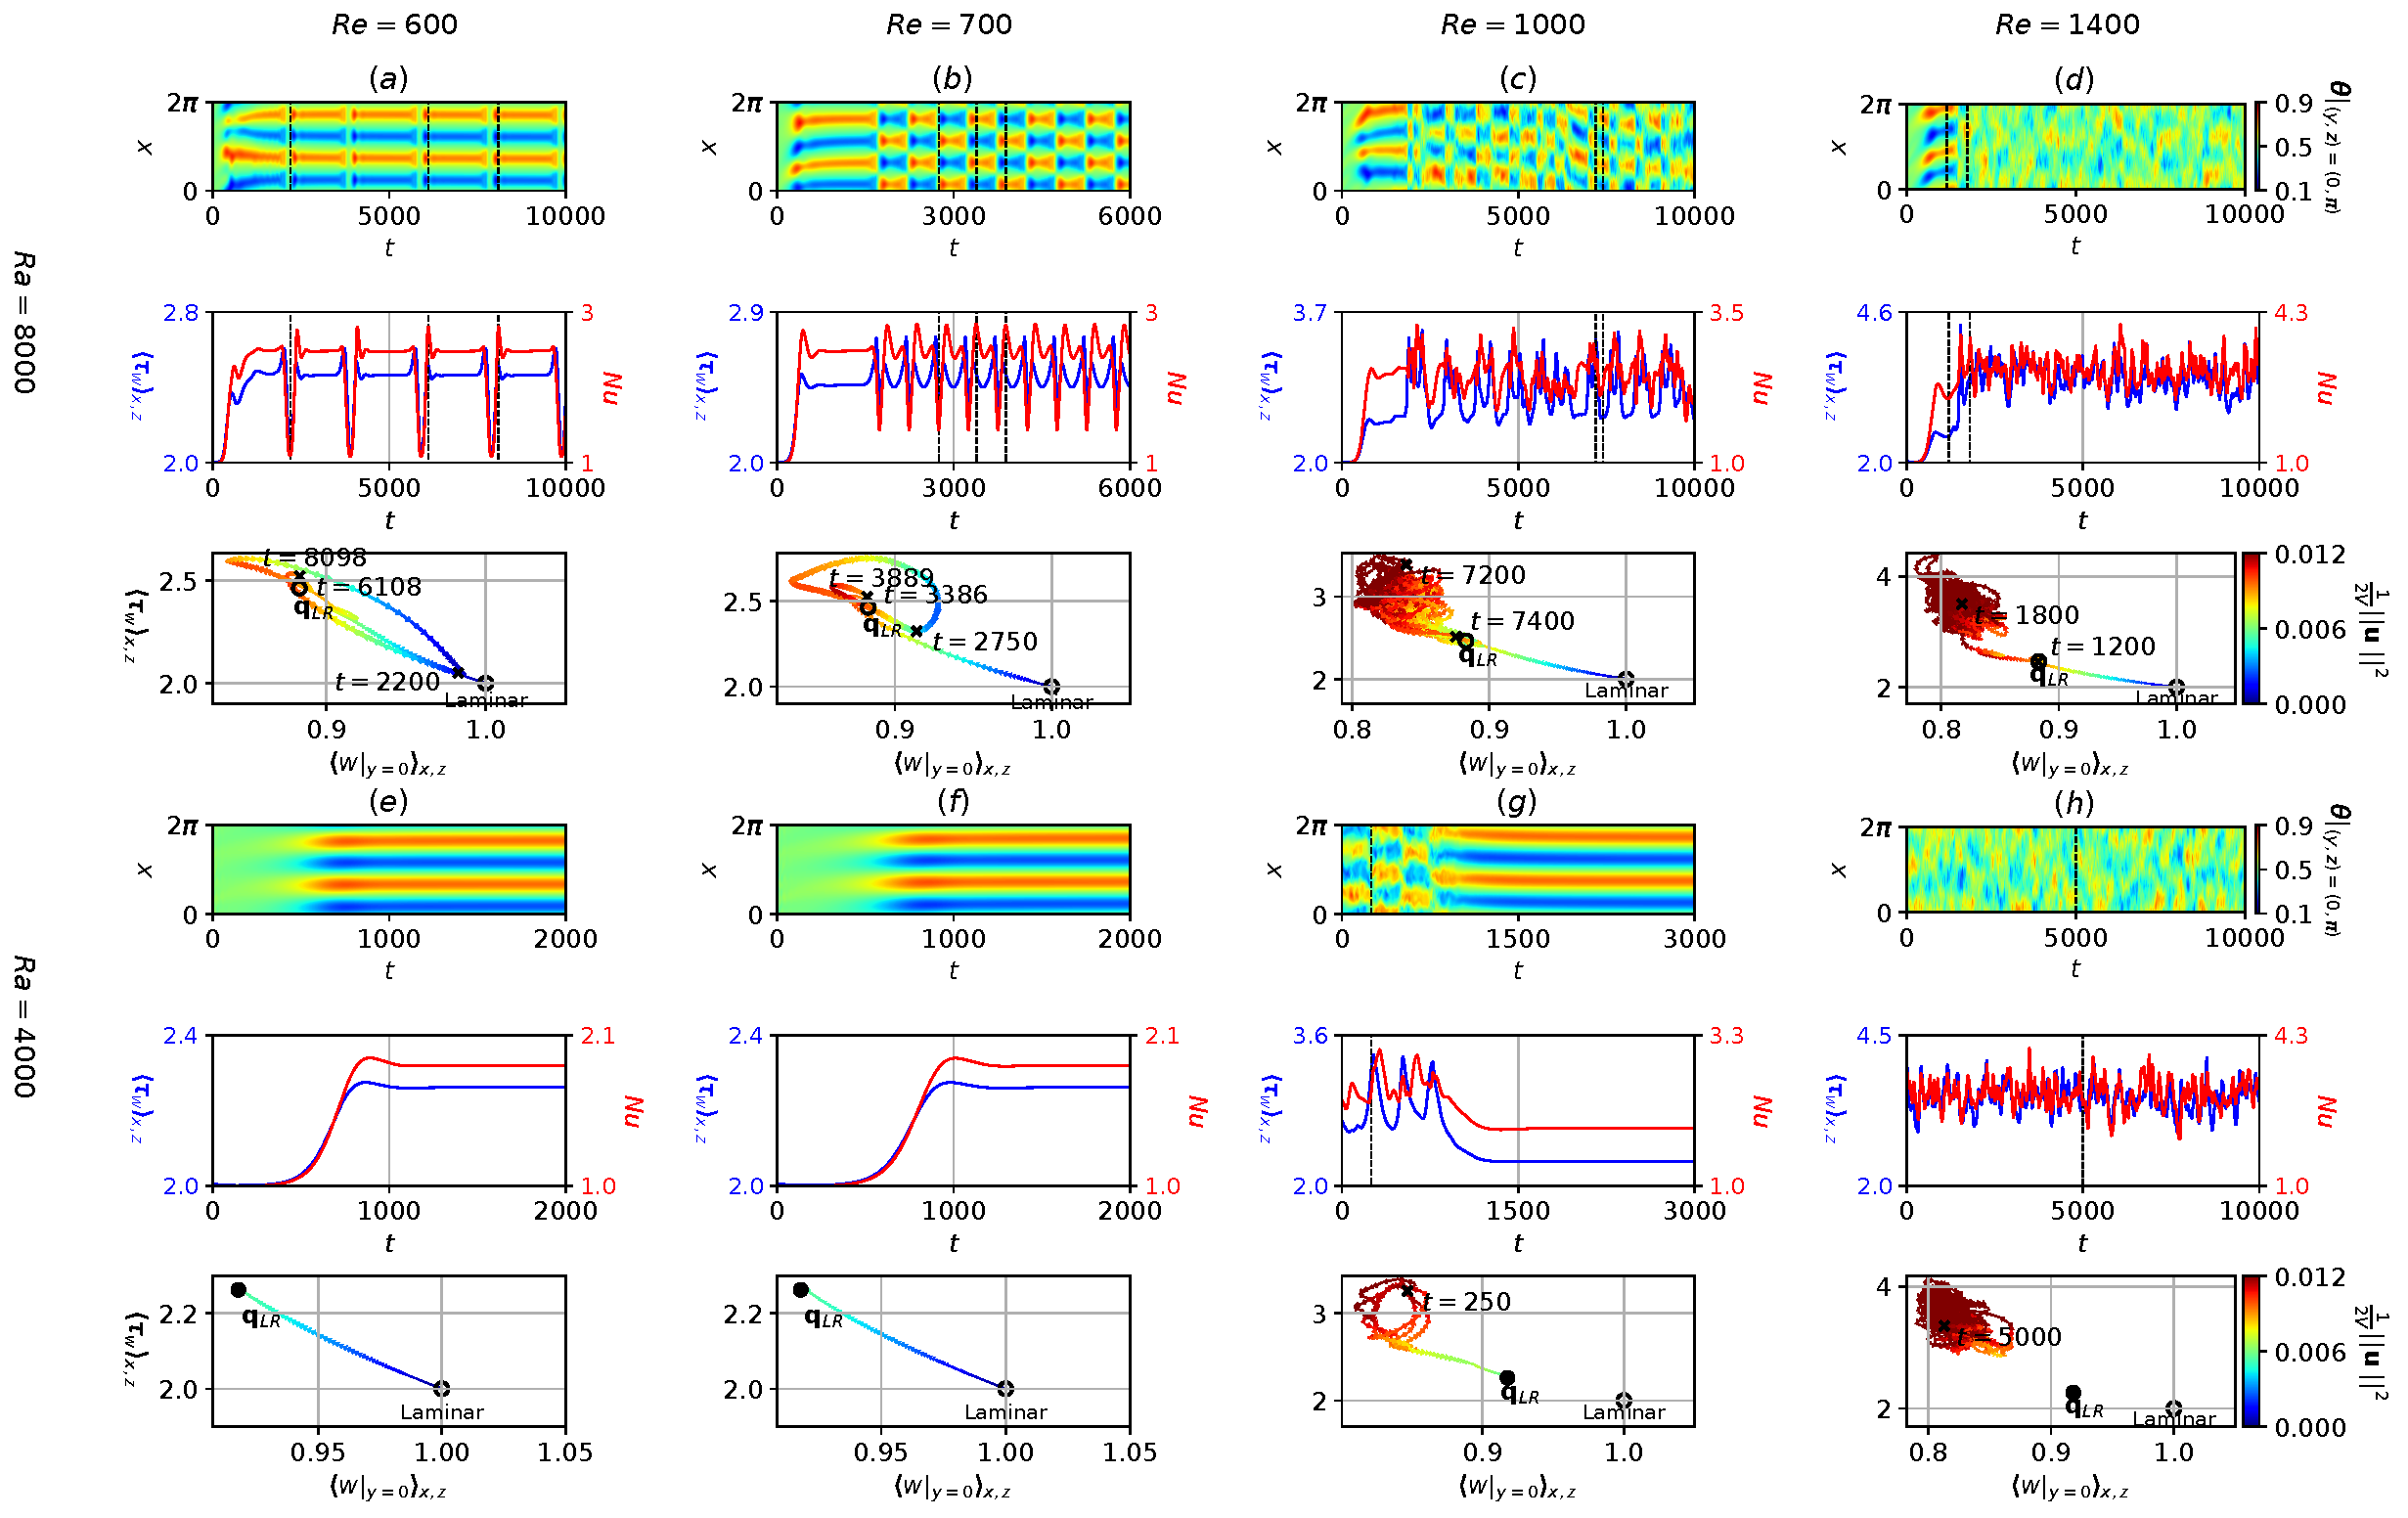
\includegraphics[width=1.35\linewidth, angle=90]{TransitionalRBP/Figures/RaEffectOnTurbulence/ConsolidatedPlot-temporal-landscape.pdf}
\caption{The behaviour of the unstable and stable longitudinal rolls at $Ra = 8000, 4000$ for (a,e) $Re = 600$, (b,f) $Re = 700$, (c,g) $Re = 1000$ and (d,h) $Re = 1400$ within $\Gamma = \pi/2$. Each parameter combination consists of three panels, depicting the (top) midplane temperature space-time plot, (mid) time history of the Nusselt number and shear, and (bottom) state space projection based on the planar averaged centerline velocity and shear, coloured by the volume normalised perturbation kinetic energy.}
\label{fig:dynamical-process}
\end{figure}
In this section, we further explore the behaviour of the \emph{TASP} as $Re$ and $Ra$ are varied.
We consider eight different cases at $Ra = 8000, 4000$ and $Re = 600, 700, 1000, 1400$.
The results of these eight cases, where longitudinal rolls are unstable at $Ra = 8000$ or stable at $Ra = 4000$, are shown in figure \ref{fig:dynamical-process}, depicting the space-time plots of the midplane temperature, $\theta|_{y=0}(x,t)$, the time history of the Nusselt number, $Nu$, and the wall shear rate, $\langle \tau_w \rangle_{x,z}$ and the state space portrait using the plane-averaged centerline velocity, $\langle w|_{y=0} \rangle_{x,z}$, the wall shear rate.
For all cases, except $Ra = 4000$, $Re = 1000$ and $Re = 1400$, their initial conditions are prepared from the laminar state, superimposed by a random noise based on a Gaussian distribution with zero mean and unit variance, scaled to a total energy of $\delta = 10^{-3}$ (see \eqref{eq:totalenergy} for the definition).
For the exceptional cases at $Ra = 4000$, $Re = 1000$ and $Re = 1400$, where subcritical turbulence and stable longitudinal rolls are expected, their initial conditions are obtained by gradually lowering $Re$ from a statistically stationary turbulent solution at $Ra = 4000, Re = 2000$.

We first consider $Re=1000$ (figures \ref{fig:dynamical-process}(c,g)). At $Ra = 8000$ (figure \ref{fig:dynamical-process}(c)), the trajectory becomes turbulent near $t=7200$, marked by large near-wall transport properties such as $Nu$ and $\langle \tau_w \rangle_{x,z}$.
The solution trajectory subsequently decays towards the longitudinal roll state, $\mathbf{q}_{LR}$ with roll wavenumber $\alpha d =4$, at $t = 7400$, before regenerating again, consistent with the \emph{TASP} in \S \ref{sec:TASP}.
As $Ra$ is lowered to $4000$ (figure \ref{fig:dynamical-process}(g)), the solution trajectory decays towards the longitudinal roll state, $\mathbf{q}_{LR}$.
In both cases, turbulence appear to be transient.
Sustained turbulence occurs only when the longitudinal rolls are linearly unstable (i.e. $Ra = 8000$), and guides the trajectory back toward turbulence. Otherwise (i.e. $Ra = 4000$), the solution ultimately relaminarises.
% In this case, the longitudinal rolls are linearly stable, confirming our hypothesis earlier that the \emph{TASP} is only established when longitudinal rolls become linearly unstable above a certain $Ra$-threshold (i.e. $Ra \gtrsim Ra_{s} \approx 4720$).

At $Re = 1400$, $Ra = 4000$, the solution trajectory remains within the turbulent `cloud' near $(0.8, 3.8)$ for $t \in [0,10000]$, as illustrated in figure \ref{fig:dynamical-process}(h).
This suggests that turbulence in this case might be an attractor sustaining indefinitely, although we have not investigated whether the turbulent chaotic saddle at $Re = 1000$ truly transitioned into an attractor at $Re = 1400$.
As $Ra$ is increased to $8000$, the solution trajectory originating from the laminar state evolves towards the unstable longitudinal roll state, $\mathbf{q}_{LR}$ at $t = 1550$, transitioning into turbulence at $t= 1800$.
Therefore, in this case, the linearly unstable longitudinal rolls serve as an intermediate transitional pathway between the laminar base state and subcritical turbulence, whereas at $Ra = 4000$, a bistability between stable longitudinal rolls (not shown) and turbulence is expected.

Next, we examine the behaviour of \emph{TASP} as $Re$ decreases towards the intermittent regime at $Re = 600, 700$, where a periodic orbit emerges between the longitudinal roll and the laminar state (figure \ref{fig:dynamical-process}(a,b,e,f)).
At $Re = 600, Ra = 8000$ in figure \ref{fig:dynamical-process}(a), the solution trajectory initially evolves towards the longitudinal roll state, $\mathbf{q}_{LR}$, which is linearly unstable and breaks down towards the laminar state at $t = 2200$.
This breakdown is evidenced by the trajectory's proximity to the laminar state in state space and the presence of a narrow green patch in the midplane temperature spacetime plot.
The longitudinal roll state is regenerated again, forming a periodic orbit with a period of $T_{period} = 8098-6108 =1990$, oscillating between the longitudinal roll and laminar state over five intervals within $t \in [0, 10000]$. 
As $Re$ increases slightly to $700$, the periodic orbit persists over a shorter period of $T_{period} = 3889 - 3386 = 503$.
A notable difference is observed in the regenerated longitudinal rolls, which are continuously translated by $L_x/2$ in the $x$-direction.
Additionally, as $Re$ increases from $600$ to $700$, the trajectory moves further away from the laminar state during breakdown, suggesting an increasing attraction towards the longitudinal roll state, $\mathbf{q}_{LR}$ (compare $t = 2200$ in figure \ref{fig:dynamical-process}(a) and $t = 2750$ in figure \ref{fig:dynamical-process}(b)).
When $Ra$ is lowered to $Ra = 4000$, the periodic orbit disappears and the trajectory stabilises into the longitudinal roll state, $\mathbf{q}_{LR}$, at $Re = 600, 700$ (figure \ref{fig:dynamical-process}(e,f)).

\begin{figure}
\centering
\includegraphics[width=1.2\linewidth, angle=90]{TransitionalRBP/Figures/RaEffectOnTurbulence/statespace-cartoon-full.pdf}
\caption{A schematic version of figure \ref{fig:dynamical-process} at $Ra = 8000$, (a) $Re = 600$, (b) $Re = 700$, (c) $Re = 1000$, (d) $Re = 1400$ and $Ra = 4000$ at (e) $Re = 600,700$, (f) $Re = 1000$, (g) $Re =1400$. The longitudinal roll is linearly unstable (saddle) at $Ra = 8000$, and is stable at $Ra = 4000$, whereas the laminar state is always linearly unstable (saddle). The blue and orange solid arrows refer to the unstable manifold of longitudinal rolls and the laminar state. The red solid lines denote the chaotic trajectories of turbulence, likely forming a chaotic saddle at $Re = 1000$ and a chaotic attractor at $Re = 1400$. The black-dashed trajectories refer to possible solution trajectories, forming a periodic orbit (P.O) at $Ra = 8000$, $Re = 600, 700$, and a basin of attraction (B.o.A) at $Ra = 8000, Re = 1000$. We note that invariant states could exist at $Ra = 4000, Re = 600,700$, labelled as saddles here \citep{paranjape_direct_2023}.}
\label{fig:statespacesketch}
\end{figure}

To summarise the dynamical processes identified in figure \ref{fig:dynamical-process}, we present a schematic sketch in figure \ref{fig:statespacesketch}.
At $Ra = 8000$, $Re = 600$ and $Re= 700$, the longitudinal rolls become linearly unstable, breaking down to the laminar state before being regenerated, forming a periodic orbit enclosed by black dotted paths in figures \ref{fig:statespacesketch}(a,b).
For $Re = 700$, the regenerated longitudinal roll is continuously translated by $L_x/2$, suggesting a possible merger of two periodic orbits into one as sketched in figure \ref{fig:dynamical-process}(b).
Future bifurcation studies are required to establish this, providing an avenue for future work.
As $Ra$ is lowered to $Ra = 4000$, the laminar state stabilises into the longitudinal rolls in figure \ref{fig:statespacesketch}(e).
However, the flow in this regime may contain some invariant solutions \cite[e.g][]{paranjape_direct_2023}, denoted as saddle points here.
Integrating along the unstable manifold of longitudinal roll states at $Ra= 8000, Re = 1000$ leads to transient turbulence, which eventually decays to the laminar state before regenerating the longitudinal rolls again, forming the \emph{TASP} in figure \ref{fig:statespacesketch}(c).
In contrast, at $Ra = 4000, Re = 1000$, the longitudinal rolls become linearly stable, eliminating the intermediate (orange) pathway towards turbulence.
Therefore, the transient turbulence stabilises into longitudinal rolls, as shown with the black-dashed trajectory in figure \ref{fig:statespacesketch}(f).
For $Ra = 8000, Re = 1400$, the linearly unstable longitudinal rolls provide an intermediate pathway towards turbulence from the laminar state, as sketched in figure \ref{fig:statespacesketch}(d), breaking the bistability between the laminar state and subcritical turbulence seen at $Ra = 4000$ in figure \ref{fig:statespacesketch}(g).
This difference highlights the contribution of unstable longitudinal rolls towards the transition to turbulence within $\Gamma = \pi/2$.

We have examined the dynamics of unstable longitudinal rolls, as the Reynolds number, $Re$, and the Rayleigh number, $Ra$, are varied, identifying three key dynamical processes: (1) periodic orbits between longitudinal rolls and the laminar state (figure \ref{fig:statespacesketch}(a,b)), (2) the \emph{TASP}, where transient turbulence can be sustained (figure \ref{fig:statespacesketch}(c)) and (3) an intermediate transitional pathway towards sustained turbulence (figure \ref{fig:statespacesketch}(d)).
To establish a connection between these processes and refine their transitional boundaries, we conduct a further parametric study over fifteen numerical simulations at $Ra = 4000, 6000, 10000$ and $Re = 600, 800, 900, 1200, 1400$ for $\Gamma = \pi/2$.
Figure \ref{fig:compiled-full} presents the midplane temperature space-time plot along with the time history of the wall shear rate, $\langle \tau_w\rangle_{x,z}$ and the Nusselt number, $Nu$.
For all simulations, the initial conditions are prepared from the laminar state, superimposed with a random noise based on a Gaussian distribution with zero mean and unit variance, scaled to a total energy of $\delta = 10^{-3}$ (see definition in \eqref{eq:totalenergy}).
Due to the subcritical nature of turbulence and expected stable longitudinal rolls, exceptions are made for $Ra = 4000$, $Re = 900, 1200, 1400$, where initial conditions are taken from gradually lowering $Re$ from a statistically stationary turbulent state at $Ra = 4000, Re = 2000$.
The \emph{thermally-assisted sustaining process} is highlighted in green for $Ra \in [6000, 10000]$ and $Re \in [900, 1200]$, where temporally intermittent shear and Nusselt number fluctuations are observed, accompanied by a mixture of organised and disorganised flow structures in the temperature space-time plots.
Here, longitudinal rolls provide an intermediate pathway towards transient turbulence.
For the same $Re$ and as $Ra$ lowers to $4000$, transient turbulence eventually decays into stable longitudinal rolls labelled as `transient turbulence' in figure \ref{fig:compiled-full}.
Periodic and quasi-periodic orbits between longitudinal rolls and the laminar state appear for $Ra =  10000$, $Re = 600, 800$ and $Ra = 6000$, $Re = 800$, establishing threshold values of $Ra$ and $Re$ shaded in yellow.
Below this threshold, solutions stabilise into longitudinal rolls shaded in red.
Although longitudinal rolls are linearly stable at $Ra = 4000, Re = 1400$, turbulence is sustained at least for a sufficiently long time, shaded blue at $Re = 1400$ and labelled as `sustained turbulence' in figure \ref{fig:compiled-full}.
In this case, a bistable system forms between longitudinal rolls and turbulence at $Ra = 4000$, while longitudinal rolls provide an intermediate pathway to turbulence for $Ra \geq 6000$.

\begin{figure}
    \centering
    \includegraphics[width=1.35\linewidth, angle=90]{TransitionalRBP/Figures/RaEffectOnTurbulence/ConsolidatedPlot-full-minimal-annotated.pdf}
    \caption{The temperature space-time plots and time history of $(\tau_w, Nu)$, for $Ra \in [5000, 10000]$, $Re \in [600, 1400]$ within $\Gamma = \pi/2$. Unstable longitudinal rolls lead to the onset of (1) periodic orbits (yellow), (2) the \emph{thermally-assisted sustaining process} (green), and (3) sustained turbulence (blue), occurring beyond an $Ra-Re$ boundary, below which longitudinal rolls remain stable (red).}
    \label{fig:compiled-full}
\end{figure}

\subsection{Extending to large domains, $\Gamma = 4\pi$.}
\begin{figure}
    \centering
    \includegraphics[width=1.3\linewidth, angle=90]{TransitionalRBP/Figures/RaEffectOnTurbulence/Ra10000-MidSpaceTimeAndPDFs-landscape.pdf}
    \caption{The midplane temperature space-time plot, and near-wall wall-normal and spanwise perturbation kinetic energy normalised by the thermal velocity scale, $u_\kappa$, and the probability density functions based on planar-averaged centerline velocity and the midplane temperature for $Ra = 10000$ at (a) $Re = 500$, (b) $Re = 750$, (c) $Re = 1000$ and (d) $Re = 1050$ at $\Gamma = 4\pi$.}
    \label{fig:Ra10k-PDFs}
\end{figure}

In this section, we return to the simulation results in the large domain $\Gamma = 4\pi$ and show that many important flow features can be well explained by the confined domain $\Gamma=\pi/2$. It should be mentioned that, by doing so, the discussion in this section does not fully account for the spatial interactions between the flow structures. However, we will see that many important flow features can be well explained based on the simulation results from the confined domain. The understanding of the full spatio-temporal dynamics is deemed to be a formidable task at this point and is beyond the scope of this study. 

Here, we will focus on $Re = 500, 750, 1000, 1050$ for $Ra = 10000$ presented in figure \ref{fig:Ra10k-PDFs}, illustrating their space-time plots of the midplane temperature, $\theta|_{(y,z)=(0,8\pi)}$, and the near-wall wall-normal and spanwise perturbation kinetic energy, $\mathcal{E}_{u'+v'}$, at $y^+=15$. 
Furthermore, to statistically characterise the flow structures, we calculate the joint probability distribution function (PDF) using the velocity and temperature in the midplane, $f(w|_{y=0}, \theta|_{y=0})$.

At $Ra = 10000$, $Re = 500$, the breakdown of longitudinal rolls towards the laminar state is observed, highlighted by spatially-localised green spots in the midplane temperature plots, and dark regions in the near-wall perturbation kinetic energy spacetime plot near $t = 500, 3800$ in figure \ref{fig:Ra10k-PDFs}(a).
As $Re$ increases from $500$ to $750$, the breakdown towards the laminar state remains visually apparent. 
The spatio-temporal dynamics between longitudinal rolls and the laminar state observed in the large domain in this regime are reminiscent of the stable periodic orbits identified between them in a confined domain, although the dynamics in the large domain is much more complex due to the spatial interactions between different flow structures.
There is a noticeable decrease in the number of green and dark regions between the space-time figures \ref{fig:Ra10k-PDFs}(a) and (b), suggesting fewer laminar events at $Re = 750$.
Indeed, this difference is further reflected in their PDFs, where the probability of laminar events, at $(w|_{y=0}, \theta|_{y=0}) = (1,0)$, depicted as the head of the arc-shaped PDF, decreasing in intensity from $Re = 500$ (figure \ref{fig:Ra10k-PDFs}(a)) to $Re = 750$ (figure \ref{fig:Ra10k-PDFs}(b)).
This suggests fewer laminar-state events and more occurrences of the longitudinal roll state. It is also consistent with the result from the confined domain case, where the solution trajectory becomes increasingly attracted towards the longitudinal roll state from $Re = 600$ and $Re = 700$ at $Ra= 8000$ (figures \ref{fig:dynamical-process}(a,b)).

At $Re = 1000$, we observe the coexistence of the laminar state, the longitudinal rolls, and turbulence, as can be seen from the dark, bright and very bright regions in the near-wall wall-normal and spanwise perturbation velocities in figure \ref{fig:Ra10k-PDFs}(c). 
Starting at $t = 2000$, the longitudinal rolls that appear as elongated red/blue contour strips in figure \ref{fig:Ra10k-PDFs}{\color{blue}(c)} erupt into turbulence at $t = 2500$, appearing as very bright spots in the space-time plot of near-wall perturbation kinetic energy $\mathcal{E}_{u'+v'}$ of figure \ref{fig:Ra10k-PDFs}(c).
Turbulence is transient, decaying towards the laminar state at $t = 3000$, as indicated by the dark patches.
By $t = 4000$, longitudinal rolls are regenerated, appearing as red/blue elongated contour strips in the space-time midplane temperature plot, $\theta|_{(y,z) = (0,8\pi)}$ of figure \ref{fig:Ra10k-PDFs}(c).
This process resembles \emph{TASP} in a confined domain (figure \ref{fig:statespacesketch}(c)), suggesting that a similar process may be present in the large domain.

As $Re$ approaches $Re = 1050$, turbulence appears more uniformly in space and time, as seen in figure \ref{fig:Ra10k-PDFs}(d).
The increase in turbulent events is reflected by the PDFs, where a D-shaped PDF absent in $Re = 750$, gradually increases in intensity from $Re = 1000$ to $Re = 1050$.
The lack of prolonged laminar regions, previously identified for $Ra = 0$ (figure \ref{fig:spacetime-Ra0k-Re1.05k}), highlights the role of longitudinal rolls in providing an intermediate pathway from laminar to turbulent state, identified in a small domain (figure \ref{fig:dynamical-process}(d)).
                
\section{Summary}\label{sec:rbp_5}
We conclude by summarising the key findings of the transitional RBP flow in figure \ref{fig:rarephase}, where we have identified five distinct regimes and their rough transition boundaries.
At low $Re$, the flow structures are primarily organised by buoyancy-driven convection rolls, consistent with RBC studies, including features such as the bistability between ISRs and SDC and the secondary oscillatory instability.
We have shown that SDC disappears between $0.1 < Re < 1$, and the critical $Re$ at which this occurs warrants further investigation.
At intermediate $Re$, we identify a new regime known as intermittent rolls, marked by the breakdown and regeneration of longitudinal rolls. As $Re$ approaches the onset of shear-driven turbulence, we observe the co-existence of longitudinal rolls with turbulent-laminar bands.
This highlights the importance of longitudinal rolls in spatially extended RBP flows.
Due to the enforced periodic boundary condition in our simulations, the longitudinal rolls are continuously excited, rather than convected out as in the case of impulsive disturbances \citep{carriere_convective_1999, pabiou_wavy_2005}.
In finite-length experiments, careful control of system noise will likely facilitate the occurrence of this intermittent regime.

By considering a confined domain, we showed that the linearly unstable longitudinal rolls could provide a transition mechanism towards turbulence, referred to as the \textit{thermally-assisted sustaining process (TASP)}.
Finally, we examined how the \textit{TASP} mechanism evolves as $Ra$ and $Re$ vary and discussed its implications for spatially extended domains.
Further work may include a bifurcation analysis study of the \textit{TASP} within confined domains and minimal band unit, establishing dynamical connections between invariant solutions where large spatial intermittency structures are expected to be important in the transitional regime \citep{tuckerman_patterns_2020}.
